\chapter{Σχετική βιβλιογραφία}

Στο κεφάλαιο αυτό παρουσιάζουμε σχετικές προσεγγίσεις και υλοποιήσεις στο πρόβλημα του αυτόματου προγραμματισμού και της παραγωγής κώδικα.
Επειδή είναι πρακτικά αναρίθμητες, θα επικεντρωθούμε σε αυτές που είναι σχετικές με τα αναδραστικά νευρωνικά δίκτυα και σε κάποιες που παρουσιάζουν ιδιαίτερο ενδιαφέρον.

\section{\en{Generating Sequence with Recurrent Neural Networks}}
Στην εργασία των \en{Graves et al.} παρουσιάζεται πως απλές δομές αναδραστικών νευρωνικών δικτύων με στοιχεία μνήμης \en{LSTM} μπορούν να χρησιμοποιηθούν για να παράξουν σύνθετες ακολουθίες, απλά προβλέποντας ένα στοιχείο της ακολουθίας τη φορά. 
Θεωρώντας τις προβλέψεις στοχαστικές, καινούριες ακολουθίες μπορούν να προκύψουν από ένα εκπαιδευμένο δίκτυο, δειγματοληπτώντας επαναληπτικά από την έξοδο του δικτύου και ύστερα ξανά-δίνοντας ως είσοδο στο δικτύου την δειγματοληπτημένη πρόβλεψη.
Με μία διαφορετική διατύπωση, αφήνουμε το δίκτυο να αντιμετωπίσει τις επινοήσεις του ως αληθινές, περίπου σαν έναν άνθρωπο ο οποίος ονειρεύεται. 
Αν και το σύστημα είναι ντετερμινιστικό, η στοχαστικότητα που εισάγεται δειγματοληπτώντας δημιουργεί μία κατανομή σε σχέση με τις ακολουθίες.
Αυτή η κατανομή είναι δεσμευμένη, αφού η εσωτερική αναπαράσταση του δικτύου, άρα και κατανομή προβλέψεων του, εξαρτάται από τις προηγούμενες εισόδους.

Η προσέγγιση αυτή επιδεικνύεται για κείμενο (όπου οι τιμές είναι διακριτές) και για <<\en{online}>>  χειρόγραφο κείμενο (όπου οι τιμές είναι πραγματικές).
Με τον όρο <<\en{online}>> εννοούμε ότι η γραφή αποτυπώνεται ως ακολουθία διανυσμάτων θέσης ενός μολυβιού -- σε αντίθεση με το <<\en{offline}>> στο οποίο έχουμε διαθέσιμη ολόκληρη την εικόνα του χειρόγραφου.
Το σύστημα που χρησιμοποιείται είναι μια συστάδα που αποτελείται από 7 επίπεδα αναδραστικών νευρωνικών δικτύων με 700 στοιχεία μνήμης \en{LSTM}.
Για την παραγωγή ακολουθιών κειμένου χρησιμοποιούνται τρία διαφορετικά σετ δεδομένων. Το Penn Treebank και το Wikipedia Hutter Prize για το γραπτό κείμενο και το <<\en{IAM online handwriting database}>>.
Το μοντέλο καταφέρνει να παράξει ακολουθίες τόσο ρεαλιστικές ώστε να είναι συχνά δύσκολο να τις ξεχωρίσει κανείς από πραγματικές, τουλάχιστον σε πρώτη όψη.
Στα αποτελέσματα είναι ορατή μια μεγάλης εμβέλειας δομή και συνοχή.

\begin{figure}[tph]
	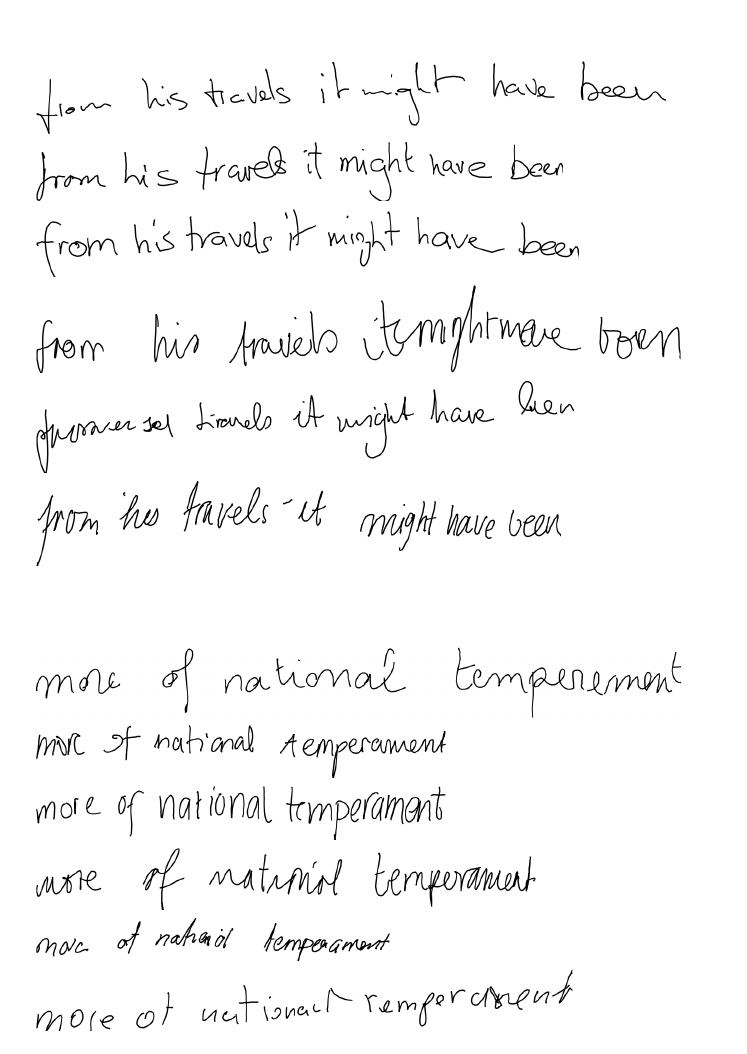
\includegraphics[width=\textwidth, keepaspectratio]{images/handwriting.png}
	\centering 
	\caption{Ένα τυπικό δομικό διάγραμμα επιτηρούμενης εκμάθησης.}
	\label{fig:training}
\end{figure}

Επιπρόσθετα, βασισμένοι στην προηγούμενη δομή, οι \en{Graves et al.} σχεδιάζουν ένα σύστημα παραγωγής χειρόγραφου κειμένου το οποίο μπορεί να γράψει αυτό που του ζητάμε.
Αυτό γίνεται με την προσθήκη ενός διανύσματος της πρότασης που θέλουμε να γράψουμε, το οποίο δίνεται στο σύστημα πρόβλεψης την ώρα της παραγωγής, αφού προφανώς εκπαιδευτεί σε σχετικά προβλήματα.
Η απόφαση για το πότε και πως θα γραφεί κάθε χαρακτήρας αφήνεται στο νευρωνικό δίκτυο και τα αποτελέσματα είναι αρκετά ικανοποιητικά ώστε να είναι και πάλι δύσκολο να διακριθεί αν τα <<χειρόγραφα>> ανήκουν σε κάποιον άνθρωπο ή στο σύστημα.

\section{\en{Inferring Algorithmic Patterns with Stack-Augmented Recurrent Nets}}

Οι \en{Joulin et al.} στην έρευνα τους εξετάζουν τα όρια των \en{"state of the art" Deep Learning} προσεγγίσεων.
Πιο συγκεκριμένα, εξετάζονται τα απλούστερα προβλήματα πρόβλεψης ακολουθιών που είναι πέρα από τις δυνατότητες εκμάθησης των τυπικών αναδραστικών δικτύων: αλγοριθμικά παραγμένες ακολουθίες που μπορούν να μαθευτούν μόνο από συστήματα με δυνατότητα μνήμης και απαρίθμησης.
Για παράδειγμα η σχέση $a^nb^n, n > 0$ μπορεί να παράξει την ακολουθία \en{aab\textbf{ba}aab\textbf{bba}b\textbf{a}aaaab\textbf{bbbb}}, όπου με έντονη γραμματοσειρά σημειώνονται τα στοιχεία της ακολουθίας που μπορούν να προβλεφθούν ντετερμινιστικά.

Εξετάζονται 4 διαφορετικά μοντέλα: ένα απλό αναδραστικό νευρωνικό δίκτυο, ένα \en{RNN} με στοιχεία μνήμης \en{LSTM} και 2 \en{RNN} με εξωτερική μνήμη.
Η εξωτερική μνήμη είναι για το ένα μοντέλο μια διπλά συνδεδεμένη λίστα και για το άλλο μοντέλο μια στοίβα. Όλα τα μοντέλα εκπαιδεύονται με τον αλγόριθμο \en{SGD}.
Τα μοντέλα με την εξωτερική μνήμη μαθαίνουν να χρησιμοποιούν τις θεωρητικά απείρου μήκους εξωτερικές μνήμες τους, με στοιχειώδεις εντολές (\en{push, pop, insert, no-op}). 

Τελικώς δείχνουν πως μερικοί βασικοί αλγόριθμοι μπορούν να μαθευτούν από ακολουθιακά δεδομένα χρησιμοποιώντας \en{RNNs} με μνήμη. Τα μοντέλα με εξωτερική μνήμη ξεπερνούν σε επιδόσεις τα υπόλοιπα μοντέλα. Οι συγγραφείς υποσημειώνουν πως είναι σημαντικό να μεγαλώσουμε την πολυπλοκότητα του μοντέλου με δομημένο τρόπο και πως η δομή των νευρωνικών δικτύων θα πρέπει να μαθαίνεται από τα δεδομένα και να μην προαποφασίζεται.

\section{\en{A Synthetic Neural Model for General Purpose Code Generation}}

Στην έρευνα τους, οι \en{Yin et al.} ασχολούνται με την αυτόματη μετατροπή εντολών φυσικής γλώσσας σε πηγαίο κώδικα γλωσσών γενικής χρήσης.
Σε αντίθεση με την πλειοψηφία των μεθόδων που απαντώνται στην βιβλιογραφία, που αντιμετωπίζουν το πρόβλημα χωρίς να λαμβάνουν υπ' όψιν την γραμματική της τελικής γλώσσας, οι ερευνητές προτείνουν ένα μοντέλο στο οποίο η γραμματική είναι γνωστή \en{a priori}.

Το συντακτικά-οδηγούμενο νευρωνικό μοντέλο παραγωγής κώδικα που προτείνεται βασίζεται σε ένα γραμματικό μοντέλο που ορίζει την παραγωγή ενός \en{Abstract Syntax Tree} σε ακολουθίες στοιχειωδών δράσεων.
Οι δράσεις αυτές χωρίζονται κανόνες παραγωγής κώδικα και σε εντολές.
Με αυτό τον τρόπο το μοντέλο δε χρειάζεται να μάθει την γραμματική από τα περιορισμένα σε ποσότητα δεδομένα εκμάθησης.
Το αναδραστικό νευρωνικό δίκτυο που χρησιμοποιείται βασίζεται σε στοιχεία \en{LSTM} με τροποποίηση, ώστε να λαμβάνεται υπ' όψιν η αναδρομική φύση των γλωσσών προγραμματισμού.
Η δομή του συστήματος γίνεται σύμφωνα με αρχιτεκτονική \en{encoder-decoder RNN with attention} \cite{Bahdanau2014}, τεχνική η οποία γνωρίζει μεγάλη χρήση και επιτυχία τα λίγα χρόνια ύπαρξης της.
Για την εκπαίδευση <<δείχνουμε>> στο νευρωνικό κομμάτια κώδικα, μετατρέπονται σε \en{ASTs}και από εκεί σε κώδικα σύμφωνα την γραμματική που υποδεικνύεται.

Το μοντέλο ξεπερα τις \en{state of the art} προσεγγίσεις νευρωνικών δικτύων των Ling και των Dong\cite{} and Lapata\cite{} στο \en{Hearthstone dataset} με παραγόμενη γλώσσα την \en{Python}.
Συμπεραίνεται έτσι, η σημαντικότητα της γραμματικής της γλώσσας σε σχέση με τις επιδόσεις. 

\section{\en{End-to-End Memory Networks}}

Οι Sukhbaatar et al., παρουσιάζουν ένα ευέλικτο νευρωνικό μοντέλο με μεγάλη εξωτερική μνήμη. 
Το μοντέλο σε αντίθεση με αντίστοιχες εργασίες δικτύων με μνήμη εκπαιδεύεται <<\en{end-to-end}>>, που, στα πλαίσια της εκπαίδευσης μοντέλων νευρωνικών δικτύων, σημαίνει πως το μοντέλο εκπαιδεύεται σε μια ενιαία διαδικασία και απλά του δίνονται οι είσοδοι και οι σωστές έξοδοι, χωρίς επιπρόσθετη εργασία για δημιουργία και ρύθμιση χαρακτηριστικών. Οι επιδόσεις του συστήματος εξετάζονται σε προβλήματα συνθετικών ερωταπαντήσεων και σε προβλήματα μοντελοποίησης φυσικής γλώσσας.

Το σύστημα δέχεται ένα σετ εισόδων, μια ερώτηση και εξάγει μία απάντηση. 
Το σετ εισόδων αποθηκεύεται στη μνήμη σε μορφή εσωτερικών αναπαραστάσεων. Για κάθε ερώτηση υπολογίζεται ένας δείκτης που εκφράζει κατά πόσο αντιστοιχεί η ερώτηση με τα στοιχεία της μνήμης.
Από τις εισόδους, επιπρόσθετα, υπολογίζεται και μία αναπαράσταση της αναμενόμενης εξόδου.
Η τελευταία σε συνδυασμό με τον δείκτη συσχέτισης ερώτησης-μνήμης χρησιμοποιείται για την εξαγωγή της τελικής απάντησης. Ολόκληρο το σύστημα είναι παραγωγίσιμο, οπότε μπορούμε να χρησιμοποιήσουμε τις τυπικές μεθόδους για την εκμάθηση του.

Για να εξετάσουμε τις επιδόσεις στην μοντελοποίηση φυσικής γλώσσας (με την οποία ασχολούμαστε επειδή βρίσκεται πιο κοντά στο πρόβλημα του αυτόματου προγραμματισμού) χρησιμοποιούμε τα \en{Penn Treebank Dataset} και \en{Text8 dataset}. Το δίκτυο μνήμης το οποίο εξετάσαμε ξεπερνά σε επιδόσεις διατάξεις \en{RNN} και \en{LSTM}. Αξιοσημείωτο είναι πως το νευρωνικό μοντέλο μνήμης έχει σημαντικά λιγότερες παραμέτρους από το αντίστοιχο \en{LSTM}. Σε ακόμα ένα πείραμα, έτσι, υποδεικνύεται η σημαντικότητα ύπαρξης εξωτερικής μνήμης στις διατάξεις εκμάθησης.

\section{\en{Neuro Symbolic Program Synthesis}}

Στην έρευνα τους οι \en{Parisotto et al.} ασχολούνται με ένα νευρωνικό μοντέλο σύνθεσης προγραμμάτων με σκοπό την επεκτασιμότητα και την εύκολη εξέταση της ορθότητας του παραγώμενου μοντέλου.
Σε αντίθεση με την πλειοψηφία των προσεγγίσεων στη σύγχρονη βιβλιογραφία, όπου ο χώρος αναζήτησης είναι σύμβολα της γλώσσας την οποία παράγουμε, εδώ, ο χώρος αναζήτησης είναι υποπρογράμματα που μαθαίνει το σύστημα κατά τη διάρκεια της μάθησης. Το όνομα που δίνεται στο υποσύστημα παραγωγής είναι \en{Recursive-Reverse-Recursive Neural Network (R3NN)}.


Το υποσύστημα παραγωγής εξάγει αναπαραστάσεις υποπρογραμμάτων σε μορφές δέντρων, στις οποίες κάθε στοιχείο είναι είτε κανόνας παραγωγής είτε σύμβολο, διαδικασία η οποία χωρίζεται σε 3 μέρη.
Αρχικά δεδομένου ενός τέτοιου δέντρου, δίνεται ένα διάνυσμα αναπαράστασης σε κάθε φύλλο του.
Ύστερα, το δέντρο διαβάζεται προς τα πάνω, ώστε να δοθεί μία αναπαράσταση ολόκληρου του δέντρου στη ρίζα του.
Τέλος επαναλαμβάνεται το προς τα κάτω πέρασμα ώστε να δοθεί σε κάθε φύλλο μια αναπαράσταση ολόκληρου του δέντρου.
Με αυτό τον τρόπο κάθε φύλλο έχει πληροφορία για τα υπόλοιπα φύλλα και για την συνολική λειτουργικότητα του δέντρου. Τα προγράμματα στο σετ δεδομένων χωρίζονται σε στοιχειώδη βήματα για να επεξεργαστούν με τον τρόπο που περιγράψαμε παραπάνω. Τα δεδομένα εκπαίδευσης σε αυτή την περίπτωση αποτελούνται από αναπαραστάσεις εισόδων και εξόδων που δίνονται στο σύστημα παραγωγής με σε κάθε φύλλο του δέντρου.

Το σύστημα εξετάζεται στη δημιουργία προγραμμάτων διαχείρισης αλφαριθμητικών ακολουθιών. Καταφέρνει σε ένα βαθμό και να επεκτείνει προγράμματα που ήδη έχει <<δει>> ώστε να συμπεριλαμβάνουν καινούρια ζευγάρια εισόδου εξόδου αλλά και να δημιουργήσει καινούρια προγράμματα για καινούριου είδους ζευγάρια εισόδου εξόδου. Η επεκτασιμότητα που παρουσιάζει το σύστημα αυτό, με την έννοια ότι μπορεί να ξεκινήσει από κάποια προγράμματα και ύστερα να τα εμπλουτίσει είναι ένα σημαντικό και αισιόδοξο στοιχείο στην κατεύθυνση του αυτόματου προγραμματισμού. 
